\documentclass[xetex, onlymath]{beamer}
\usefonttheme{serif}
\usetheme{hsr}

% select font
\usepackage[T1]{fontenc}
\usepackage[usefilenames]{plex-otf}
\renewcommand*\familydefault{\sfdefault}

\usepackage{booktabs}
\usepackage{array}

\usepackage{listings}
%% create a lstlisting style
\lstdefinestyle{samplestyle}{
    belowcaptionskip=\baselineskip,
    breaklines=true,
    frame=none,
    inputencoding=utf8,
    % margin
    xleftmargin=\parindent,
    % numbers
    numbers=left,
    numbersep=5pt,
    numberstyle=\ttfamily\footnotesize\color{hsr-black40},
    % background
    backgroundcolor=\color{hsr-lightgrey20},
    % default language:
    language=[LaTeX]TeX,
    showstringspaces=false,
    % font
    basicstyle=\ttfamily\small,
    identifierstyle=\color{hsr-black},
    keywordstyle=\color{hsr-blue},
    commentstyle=\color{hsr-black40},
    stringstyle=\color{hsr-mauve80},
}

%% and set the chosen style
\lstset{style=samplestyle, escapechar=`}


% metadata
\title{\textrm{\LaTeX} Workshop}
\author[NaoPross]{Naoki Pross \texttt{<npross@hsr.ch>}}
\date{\today}

\institute[HSR]{Hochschule f\"ur Technik Rapperswil}
%\logo{\includegraphics[width=3cm]{figs/hsr-logo}}

\AtBeginSection[]
{
  \begin{frame}
    \frametitle{Table of Contents}
    \tableofcontents[currentsection]
  \end{frame}
}


\begin{document}
\begin{frame}
\maketitle
\end{frame}

\begin{frame}{Goal: Learn to typeset something like this}
	\begin{center}
		\vspace{1cm}
		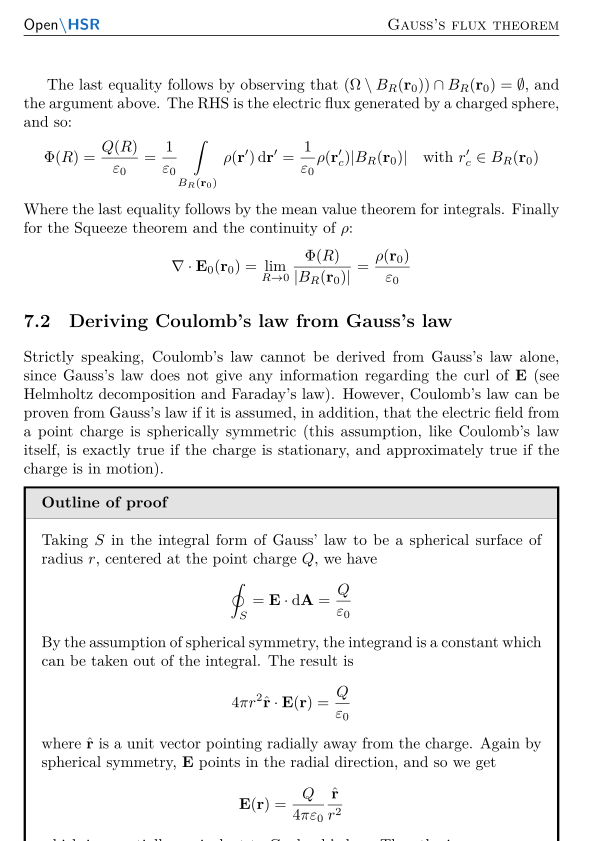
\includegraphics[width=.8\linewidth]{figs/gauss-flux}
	\end{center}
\end{frame}

\section{Introduction}

\begin{frame}{What is Typesetting}
\end{frame}

\begin{frame}{History \& \textrm{\LaTeX}}
\end{frame}

\section{Fundamentals}
\begin{frame}{Source code spacing}
\end{frame}

\begin{frame}{Special characters}
\end{frame}

\begin{frame}{Commands}
\end{frame}

\begin{frame}{Environments}
\end{frame}

\begin{frame}{Document structure}
\end{frame}

\begin{frame}{Spacing and newlines}
\end{frame}

\section{Basics}
\begin{frame}[fragile]{Emphasis, Bold, Italic, \ldots}
\begin{lstlisting}
This is \emph{emphatized}.
You may also use
\textbf{Bold},
\textit{Italic},
\textsf{Sans-Serif},
\textsc{SmallCaps},
\textrm{Roman},      % with serif
\texttt{Typewriter}. % monospaced
\end{lstlisting}

\begin{exampleblock}{}
This is \emph{emphatized}.
You may also use
\textbf{Bold},
\textit{Italic},
\textsf{Sans-Serif},
\textsc{SmallCaps}\footnote{The font used in this presentation does not have a smallcaps style},
\textrm{Roman} or
\texttt{Typewriter}.
\end{exampleblock}
\end{frame}

\begin{frame}[fragile]{Lists}
\begin{columns}
\begin{column}{.5\linewidth}
\begin{lstlisting}
\begin{itemize}
  \item Tomatoes
  \item Peppers
  \item Broccoli
\end{itemize}
\end{lstlisting}

\begin{lstlisting}
\begin{enumerate}
  \item Discovery coffee
  \item Get addicted
  \item Congratulations
\end{enumerate}
\end{lstlisting}
\end{column}

\begin{column}{.4\linewidth}
\begin{exampleblock}{Itemize}
	\begin{itemize}
		\item Tomatoes
		\item Peppers
		\item Broccoli
	\end{itemize}
\end{exampleblock}
\begin{exampleblock}{Enumerate}
	\begin{enumerate}
		\item Discovery coffee
		\item Get addicted
		\item Congratulations
	\end{enumerate}
\end{exampleblock}
\end{column}
\end{columns}
\end{frame}

\begin{frame}[fragile]{Description}
\begin{lstlisting}
\begin{description}
  \item[Programmer] A person who is paid to professionally scream at a computer.
  \item[Manager] A person who appears to know how all tasks should be accomplished but can't actually do any of those tasks themselves.
\end{description}
\end{lstlisting}

\begin{exampleblock}{}
\begin{description}
  \item[Programmer] A person who is paid to professionally scream at a computer.
  \item[Manager] A person who appears to know how all tasks should be accomplished but can't actually do any of those tasks themselves.
\end{description}
\end{exampleblock}
\end{frame}

\begin{frame}{Floating elements}
\begin{table}
	\caption{Floats placing permissions}
	\begin{tabular}{>{\ttfamily}l l}
		\toprule
		\textsf{Specifier} & Permission \\
		\midrule
		h & Place around here \\
		t & At the top of the page \\
		b & At the bottom of the page \\
		p & On a special page containing only floats \\
		! & ``I don't care if it will be ugly'' \\
		H\footnote{Requires the ``\texttt{float}'' package, i.e. 
			``\texttt{\textbackslash usepackage\{float\}}''} 
		  & Place \textbf{exactly here} (may look very ugly) \\
		\bottomrule
	\end{tabular}
\end{table}
\end{frame}

\begin{frame}[fragile]{Tables and tabular}
\begin{lstlisting}
\begin{table}[h]
  \caption{Not up to date numbers}
  \begin{tabular}{l r r}
    `\textcolor{hsr-mauve}{\textbackslash toprule\textsuperscript{1}}`
    Country & Infected & Deaths \\
    `\textcolor{hsr-mauve}{\textbackslash midrule\textsuperscript{1}}`
    China       & 80'652 & 3'070 \\
    South Korea &  7'041 &    44 \\
    Italy       &  5'833 &   233 \\
    `\textcolor{hsr-mauve}{\textbackslash bottomrule\textsuperscript{1}}`
  \end{tabular}
\end{table}
\end{lstlisting}
\begin{alertblock}{\textsuperscript{1} Pro Tip}
	Add ``\texttt{\textbackslash usepackage\{booktabs\}}'' to use
	rulers.
\end{alertblock}
\end{frame}

\begin{frame}{Tables and tabular}
\begin{exampleblock}{}
\begin{table}
  \caption{Not up to date numbers}
  \begin{tabular}{l r r}
    \toprule
    Country & Infected & Deaths \\
    \midrule
    China       & 80'652 & 3'070 \\
    South Korea &  7'041 &    44 \\
    Italy\footnote{Congratulations, your public health worse than Iran's}
    &  5'833 &   233 \\
    \bottomrule
  \end{tabular}
\end{table}
\end{exampleblock}
\end{frame}


\begin{frame}{Figures}
\end{frame}

\begin{frame}{Cross-References}
\end{frame}

\section{Mathematics}
\begin{frame}{Math environments}
\end{frame}

\begin{frame}{Math symbols and fonts}
\end{frame}

\begin{frame}{Equations}
\end{frame}

\begin{frame}{Spacing in math mode}
\end{frame}

\section{Bibliography management}
\begin{frame}{TheBibliography}
\end{frame}

\begin{frame}{External bibliography}
\end{frame}

\section{Extras}
\begin{frame}{Source code listings}
\end{frame}

\begin{frame}{Plots}
\end{frame}

\begin{frame}{TikZ}
\end{frame}

\end{document}